\chapter{Building cover}

The building cover is the constructive element which protects it at the top and, by extension, the supporting structure of the element itself. Before choosing the best solution for the terminal building of Bekasi-East Jakarta Airport, it is important to remember the features expected from a building cover:

\begin{itemize}
	\item Resistance and stability, the cover has to support its own weight and possible overloads due to snow, wind, etc.
	\item Atmospheric barrier outdoors, must protect from water, wind, sun.
	\item Hydrothermal insulation, a vapour barrier must be installed to prevent condensation inside the thermal insulation.
	\item Acoustic barrier, must be protected from aircraft noise and vibrations.
	\item Thermal and fire insulation.
\end{itemize}

In addition, the cover also has to be aesthetic when facing the users of airports. In other areas you never see the building covers, but in this case many customers will arrive by plane and the cover will the first thing to be seen when arriving at the airport.

	\section{Solution adopted}
In this terminal building, a metal cover with sandwich structure is chosen as the best solution. It has many advantages in front other types of covers involving the covering, supporting structure, insulation and aestheticism of both inside and outside the building. The core made of expanded polyurethane allows to obtain a fire resistance of 2 hours. In addition, these covers are able to support great bending efforts thanks to the design of the panels and its thickness. As soon as the installation is concerned, also thanks to the composite structure it has, it allows to install the cover, insulating elements and other final details in a single stage. In this way, the reduction of the costs is significant.
	
	\section{Shape and inclination of the building cover}
	
The solution adopted for the shape and inclination of the cover, taking into account the rainy climate in the region of Indonesia, is to build a mixed cover. In the centre part and concerning all the length of the pier, the cover will be curved while in the rest of the terminal an inclined cover of 5 degrees will be used.

This type of covers are the most efficient ones when evacuating water because they do not generate leak-tightness and no extra support is necessary since gravity acts on its own. Moreover, the maintenance is not so much and consequently the costs generated due to this are lower than in other kind of covers. The only disadvantage it has the impossibility of installing machinery above the cover.

	\section{Used materials}
	
Detailing cover materials, it can assumed that due to the high temperatures in Jakarta, the heat focus will be located in the outer surface of the cover and it will be necessary to protect the terminal from heat by adding a good insulator between layers.

The main structure of the sandwich-type metal cover consists of two steel faces with low thickness joined together by a central insulating core. This insulating layer is very important due to the high temperatures reached in Jakarta, which will affect by the most part at the outer layer of the cover. The interesting point here is not to transfer this heat generated to the inner steel layer and, consequently, to the interior of the terminal building.

This type of panel is self-supporting. The sides of the upper face are outlined as nerves on which a top layer is placed. To close the thermal bridge, the steel plate which form the panel are separated by a lateral tape and in the middle of this section, the insulator is found. The panels are fixed to the belt frame by means of self-tapping screws that are hidden for aesthetic reasons.

The company that will supply the cover panels is \textit{EUROPERFIL}, the number one in cover construction sector in its region since 2014. The metallic profile used is the model \textit{EUROBASE 106 CS} and its properties can be seen in the following figure:

\begin{figure}[H]
	\centering
	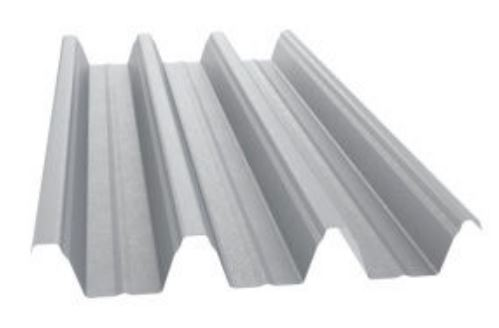
\includegraphics[clip, trim=0cm 0cm 0cm 0cm, width=0.6\textwidth]{./images/cover/profile}
	\caption{Cover steel panel used.}
	\label{profile}
\end{figure}

\begin{figure}[H]
	\centering
	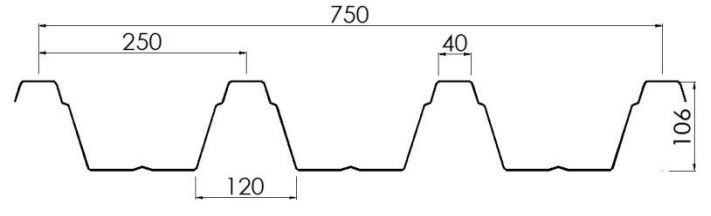
\includegraphics[clip, trim=0cm 0cm 0cm 0cm, width=0.8\textwidth]{./images/cover/profiledimension}
	\caption{Detail of the cover steel panel's section.}
	\label{profiledimension}
\end{figure}

Inside the two metallic layers of the cover, the insulator is placed. It is usually used polyurethane, expanded polystyrene or fibreglass. In addition, this structure can have an area to pass some facilities needed in the terminal building.

The thermal insulator is placed between the outer and inner plates. In this kind of systems it is advisable to use glass wool blankets because they guarantee an excellent thermal and acoustic insulation, it resists very well to fire, the installation is easy to do and they have no problem to be placed between the two steel layers. The installation of this kind of insulator will be very fast and brings flexibility since, in case of a future extension, it can be substituted by a bigger one.

The company that will supply the thermal insulation of glass wool is \textit{RSA GLASSWOOL}. It is chosen glass wool of 50 mm thick, which generates a great thermal and acoustic insulation and a total guarantee of safety in case of fire. It is supplied in form of blankets and panels with or without coating, making it feasible to be used in a wide variety of situations.

\begin{figure}[H]
	\centering
	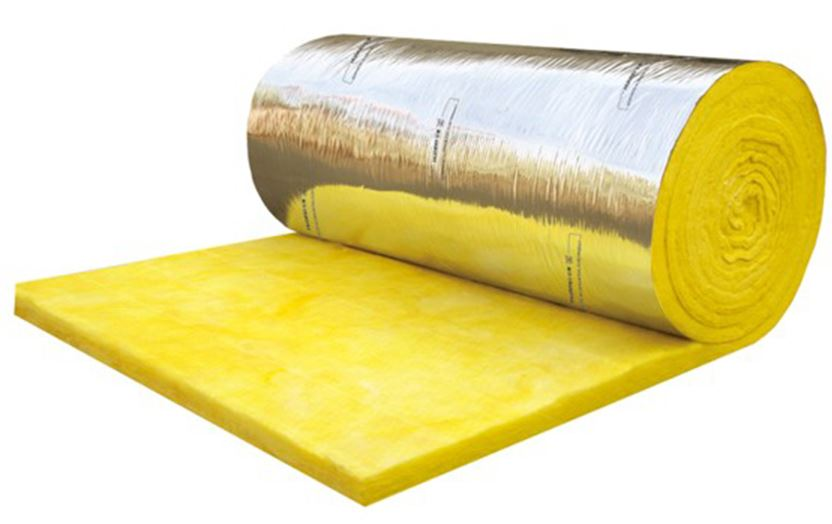
\includegraphics[clip, trim=0cm 0cm 0cm 0cm, width=0.5\textwidth]{./images/cover/glasswool}
	\caption{Insulator used between the steel panels of the cover.}
	\label{glasswool}
\end{figure}


		
	\section{Sewer system}